\documentclass[12pt]{article}


\usepackage{amssymb, amsthm, amsmath, graphicx, float, braket, fancyhdr,tabu,setspace}
\usepackage[superscript,biblabel]{cite}

\newcommand{\K}{-\frac{\hbar^2}{2 m} \nabla^2}
\newcommand{\fs}{\textforwardslash}
\newcommand{\B}{\mathbf}
\newcommand{\eq}[1]{\begin{align}#1\end{align}}
\providecommand{\e}[1]{\ensuremath{\times 10^{#1}}}
\providecommand{\us}[1]{\ensuremath{_{\textrm{#1}}}}
\providecommand{\super}[1]{\ensuremath{^{\textrm{#1}}}}
\newcommand{\ct}[1]{\cite{#1}}
\newcommand{\degree}{\ensuremath{^\circ}}
\newcommand{\tus}[1]{$_{\text{#1}}$}
\newcommand{\tls}[1]{$^{\text{#1}}$}

\addtolength{\textheight}{1.8in}
\addtolength{\voffset}{-1in}
\addtolength{\textwidth}{0.8in}
\addtolength{\hoffset}{-0.4in}

\linespread{1.3}

% \setlength\parindent{0pt} 
\setlength{\parskip}{10pt}

\bibliographystyle{unsrt}

\title{Clausius-Mossoti Factor and Dielectrophoresis Library}
\author{S. D. Sawtelle}

\begin{document}

\maketitle 

\begin{spacing}{0.5} \tableofcontents \end{spacing}
\newpage

\section{Introduction}

The goal of this code library is to facilitate making predictions regarding DEP forces on particles in different solutions and at different frequencies. This package can be used to model prokaryotic cells with membrane and cell wall, eukaryotic cells or organelles with membrane, homogeneous solid spheres such as polystyrene beads. Common needs in DEP simulation are:

\begin{enumerate}
  \item Comparing CM factor vs. frequency for different particles in the same medium
  \item Calculating crossover frequency vs. conductivity for a particle(s)
\end{enumerate}


To increase flexibility of the library I have built independent functions for each of our major particles of interest which will calculate the complex permittivity, $\epsilon^*_{p}$, given an input vector of particle parameters and an input frequency. Different functions are needed for different particles due to modeling shelled vs unshelled and spherical vs non-spherical particles. I have separated the function for finding the complex permittivity of a particle from the function for finding the CM factor to provide for flexibility for those who want to modify the code for different mathematical models of CM factor. I have also used these basic functions to code scripts for some common needs. 

\textit{A Note on Modeling Approximations}. In general a medium has a frequency-dependent complex permittivity $\epsilon^*_{m}(\omega)=\epsilon_1(\omega)-i\epsilon_2(\omega)$. In the low frequency regime of interest for DEP we can almost always take the solution to have constant $\epsilon_1$ (typically equal to that of water except in very dense media like whole blood) and assume $\epsilon_2$ is due entirely to conductive losses rather than e.g. dipole relaxations or other dissipative mechanisms. In this case, the relative complex permittivity of the solution is well modeled as $\epsilon^*_{m}=\epsilon_w-i\frac{\sigma}{\omega\epsilon_0}$, where $\sigma$ is the DC conductivity, and $\epsilon_0$ is the free space permittivity. For solutions like whole blood where there is some non-negligible frequency dependence in the range of interest, the Library scripts can still be used by feeding in a vector of experimental or simulated medium permittivies.  

\section{Library Functions}

\begin{tabular}{ | l | p{13.2cm} |}
    \hline
    \textbf{Function Handle} & \textbf{Description} \\ \hline
    DefineParams & {\footnotesize [Ecoli\_params,RBC\_params,Exosome\_params,Bead\_params]=defineParams()} 
\newline

This is where you hardcode values for geometry and complex permittivity of your particles of interest. It returns vectors of these parameters for E.Coli bacteria, red blood cells, polystyrene beads and exosomes. \\ \hline
find\textit{Particle}\_complex & {\footnotesize \textit{Particle}\_complex=find\textit{Particle}\_complex(\textit{Particle}\_params)
\newline 
[\textit{Particle}\_complex, \textit{Particle}\_depolarization]=find\textit{Particle}\_complex(\textit{Particle}\_params)} 
\newline

Here \textit{Particle} can take the value of several particles of interest. This function calculates an effective complex permittivity for the particle. A description of the mathematical model used here can be found in the 2011 Lab on a Chip
	paper "Continuous dielectrophoretic bacterial..." by Park et al.
	For non-spherical shapes the CM factor is calculated from the average
	value along each principle axis. The expression for each axis CM is slightly
	different from the standard expression, involving a depolarization factor. Consequently 
	this function must return a complex permittivity 3-vector and a  depolarization factor tensor. \\ \hline
findMed\_complex & {\footnotesize Med\_complex=findMed\_complex(sigmed,emed,f)} 
\newline

This will calculate the complex permittivity of the medium at a given frequency, using input parameters of DC conductivity and permittivity. In the scripts the use of the this function can be replaced by providing instead a vector of medium complex permittivity at different frequencies. 
\\
\hline
 find\textit{Particle}\_CM & {\footnotesize \textit{Particle}\_CM=find\textit{Particle}\_CM(\textit{Particle}\_complex, Med\_complex)
\newline 
\textit{Particle}\_CM=find\textit{Particle}\_CM(\textit{Particle}\_complex,\textit{Particle}\_depolarization,Med\_complex)} 
\newline 

This will calculate the complex CM factor from the complex permittivites of the particle and the medium. \\
    \hline
findBead\_xover & {\footnotesize xover=findBead\_xover(sigma,radius)}
\newline

This script finds the zero-crossing frequency along the CM curve for a given solution conductivity and bead radius. If there is no zero-crossing in a reasonable frequency interval, it returns 0.
 \\
    \hline

    \end{tabular}


\section{Library Scripts}

\begin{tabular}{ | l | p{11cm} |}
    \hline
    \textbf{Script Handle} & \textbf{Description} \\ \hline
CMcurves\_sigma\_Ecoli\_RBC & This script computes the real part of the CM factor and plots it as a function of frequency for a range of medium conductivities. The plots for E.coli and RBCs are separate. \\ \hline
CMcurves\_morphology\_Ecoli & This script computes the real part of the CM factor and plots it as a function of frequency for a range of Ecoli geometrical scaling parameters. This is helpful in knowing what behavior to expect from heterogeneous populations.\\ \hline
Compare\_Ecoli\_RBC & This script compares the values of the CM factor and force pre-factor for
 different particles as a function of frequency and medium conductivity.
 This will generate a heatmap illustrating the ratio between the CM
 factors or forces for the two different particles. The CM ratio heatmap
 can be interpreted as follows - when the particles experience opposite
 forces due to different sign of the CM factor, the heat map is red, when
 the forces are aligned the heatmap is green. the intensity of these
 colors represents an increasing magnitude of the CM ratio. The Force
 ratio heatmap maps the log of the ratio of the absolute values of the forces. Again, red indicates a positive value, green indicates a negative value, intensity of the respective indicates magnitude increasing from zero. The particular form for these prefactors comes
 from the wikipedia page on dielectrophoresis, the ecoli variant is for a
 field-aligned ellipsoid, the RBC are taken as spherical. The reamining
 factors in the force calculation are common between the two particles
 since they involve only the medium permittivity and the electric field
 profile. \\ \hline
Crossover\_beads & This script plots of the crossover frequency shifts as the medium
conductivity changes, and does this for several different sizes of beads.\\
\hline
\end{tabular}

\newpage

\section{Example Plots}

\begin{figure}[here]
\centering
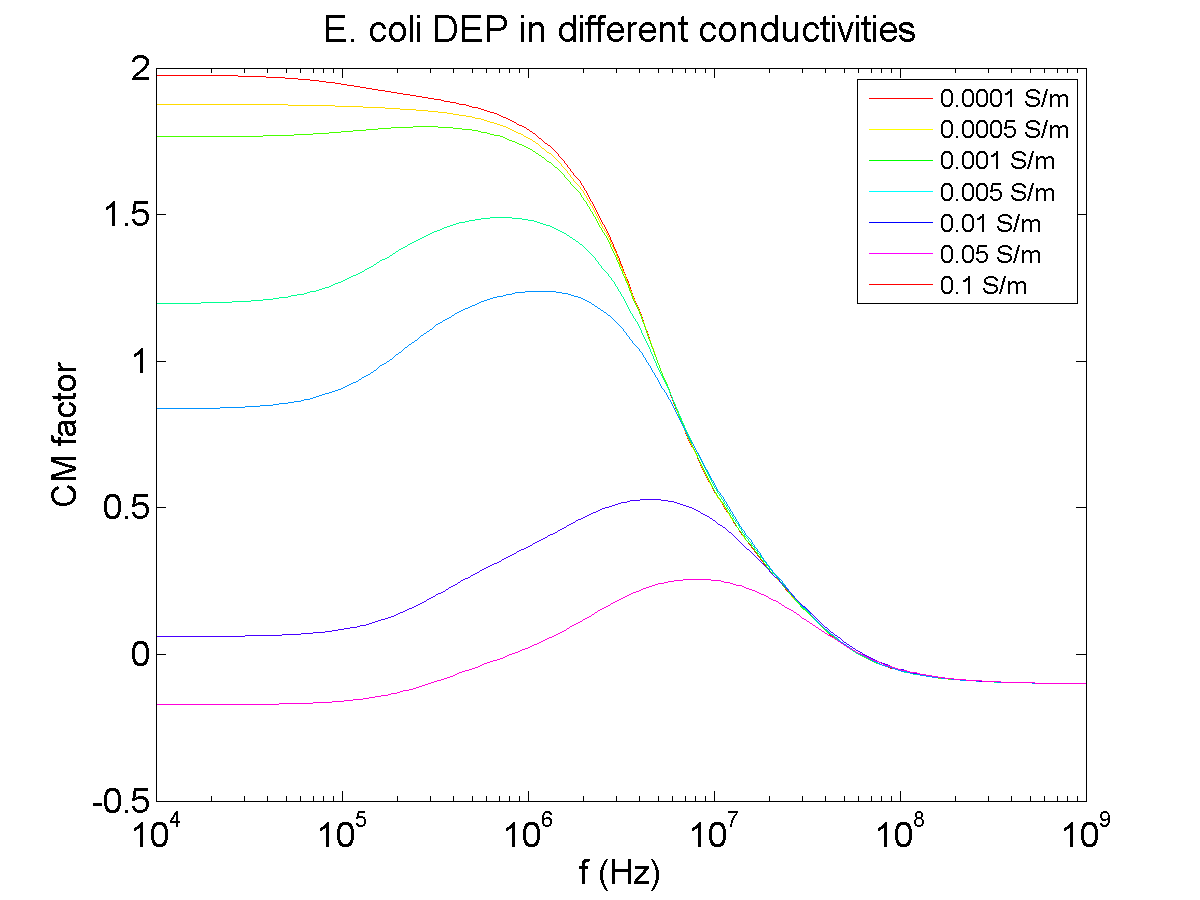
\includegraphics[width=0.7\textwidth]{Figures/CMcurves_Ecoli.png}
\caption{Generated by the CMcurves\_sigma\_Ecoli\_RBC script.}
\end{figure}

\begin{figure}[here]
\centering
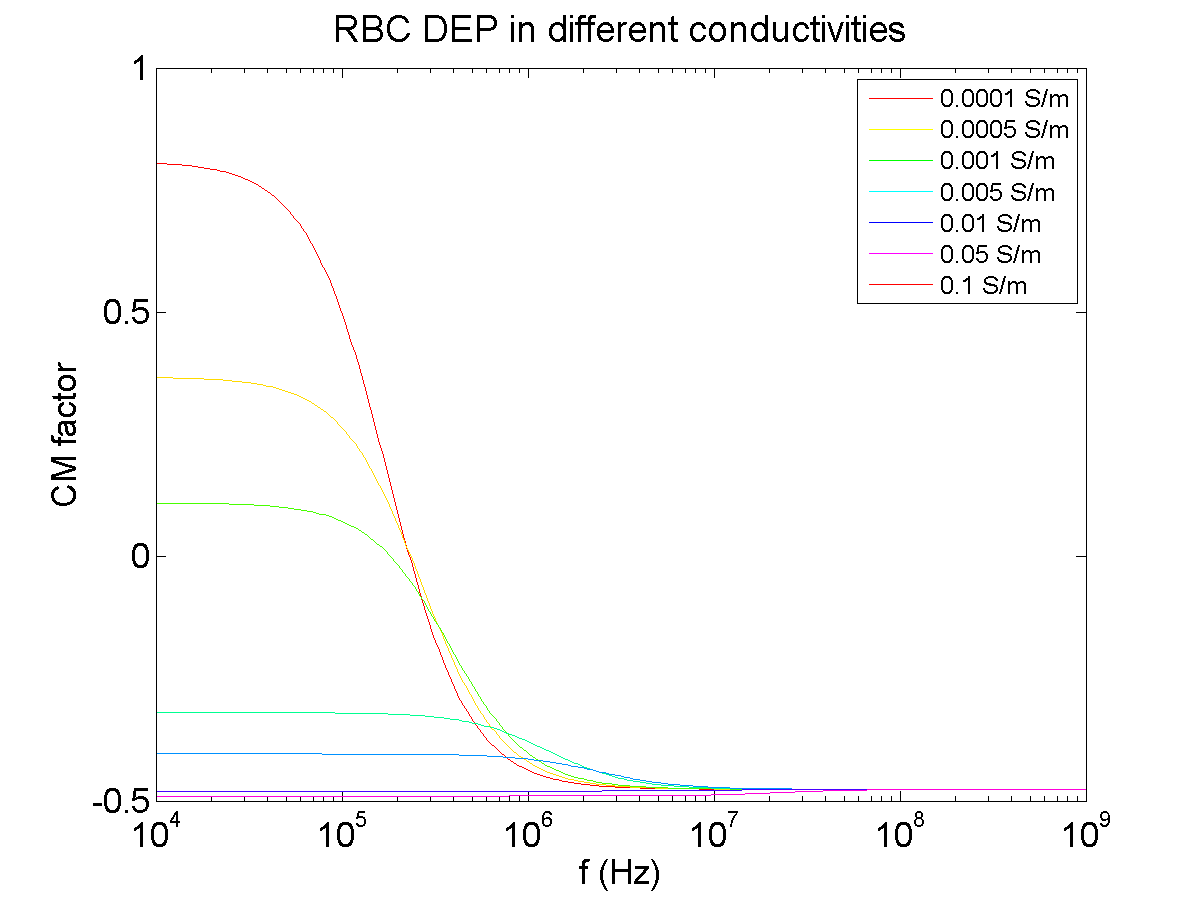
\includegraphics[width=0.7\textwidth]{Figures/CMcurves_RBC.png}
\caption{Generated by the CMcurves\_sigma\_Ecoli\_RBC script.}
\end{figure}

\begin{figure}[here]
\centering
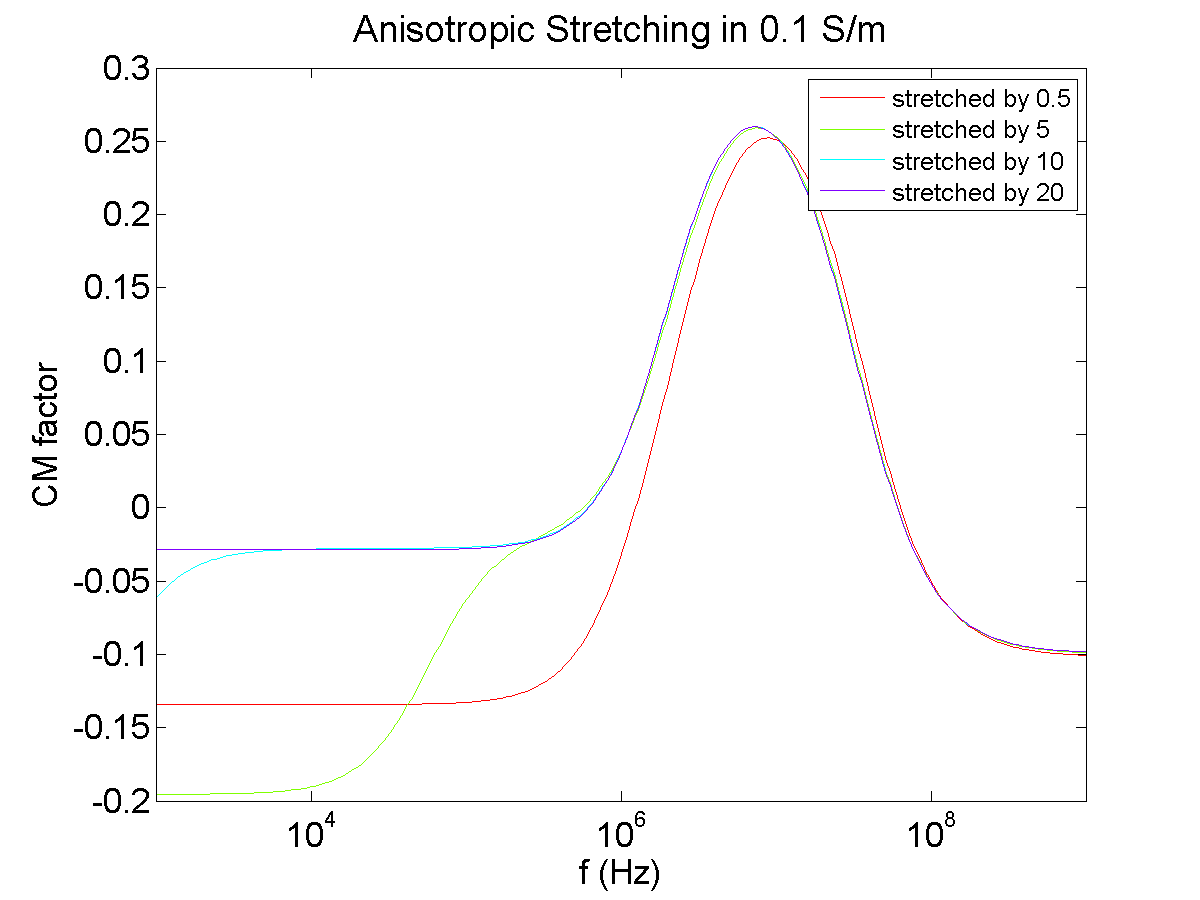
\includegraphics[width=0.7\textwidth]{Figures/CM_AnistropicStretch.png}
\caption{Generated by the CMcurves\_morphology\_Ecoli script.}
\end{figure}

\begin{figure}[here]
\centering
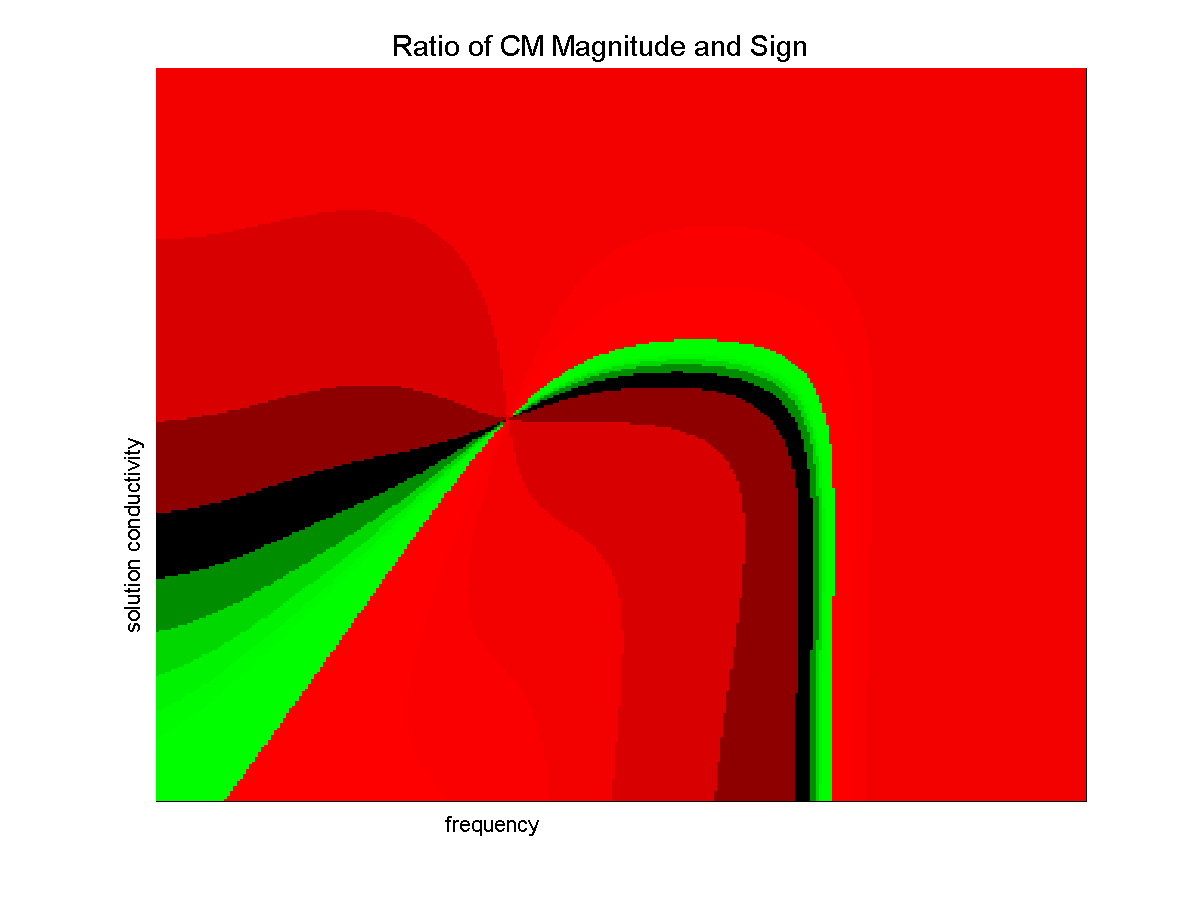
\includegraphics[width=0.7\textwidth]{Figures/CMcompare_sign_mag}
\caption{Generated by the Compare\_Ecoli\_RBC script.}
\end{figure}

\begin{figure}[here]
\centering
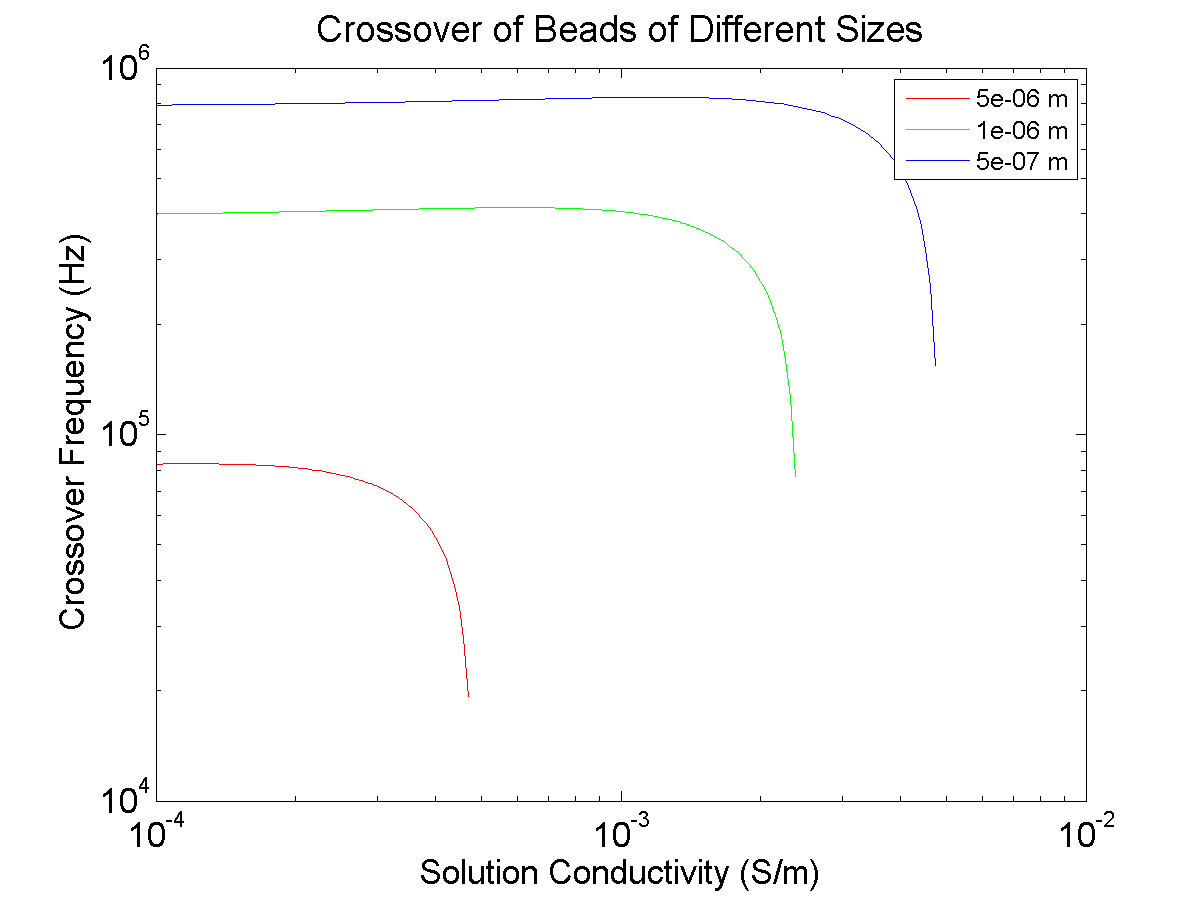
\includegraphics[width=0.7\textwidth]{Figures/Crossover_size}
\caption{Generated by the Crossover\_beads script.}
\end{figure}

%\bibliography{140211_prospectus} 

\end{document}